\section{Multi-Layer Perceptron}
La terza famiglia di modelli che abbiamo implementato è quella delle reti 
neurali, più nello specifico i Percettroni Multi-Strato (MLP).

Rispetto ai modelli già citati, le reti neurali si distinguono per il grande 
numero di parametri che possono essere impostati e per il loro effetto sulle 
performance ottenibili. L'architettura della rete, che comprende il numero di 
neuroni utilizzati, la funzione di attivazione utilizzata, il tipo di 
collegamenti tra neuroni, ha un peso importante sui risultati, ma la scelta di 
architetture ottimali resta un argomento di ricerca molto attuale.

Dopo una fase esplorativa iniziale in cui abbiamo valutato diverse 
architetture, ci siamo concentrati su una semplice architettura feed-forward 
fully-connected, composta da due hidden layer rispettivamente di 30 e 15 
neuroni. Il layer di output è composto di due neuroni, rappresentanti il valore 
target positivo e negativo. Attraverso la funzione softmax, l'output dei 
neuroni viene trasformato nel valore di probabilità usato per effettuare le 
predizioni.

Sull'ultimo hidden layer è stata applicata la tecnica del \textbf{dropout} con 
probabilità 50\%, con l'obiettivo di ridurre l'overfitting e migliorare la 
generalizzazione della rete.

Negli esperimenti abbiamo confrontato le prestazioni di due modelli basati 
sull'architettura descritta, variando la funzione di attivazione dei neuroni 
tra ReLU (vedi Equazione~\ref{eq:relu}) e sigmoide (vedi 
Equazione~\ref{eq:sigmoid}). 
\begin{align}
	ReLU(x) = \max(0, x) = \begin{cases} 
		x & \mbox{se }x > 0 \\
		0 & \mbox{altrimenti}
	\end{cases}
	\label{eq:relu}
\end{align}
\begin{align}
	sigmoide(x) = \frac{1}{1 + e^{-x}}
	\label{eq:sigmoid}
\end{align}

In Figura~\ref{fig:mlp_architecture} si possono vedere le
strutture dei modelli risultanti, visualizzate da \texttt{mxnet} attraverso la 
libreria \texttt{graphviz}.

\begin{figure}[H]
	\centering
	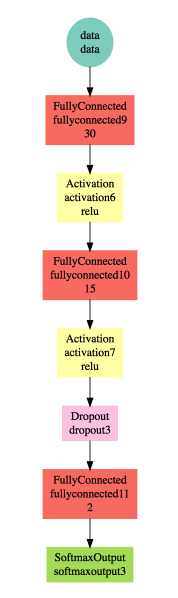
\includegraphics[width=0.2\textwidth]{images/ml/mlp/relu}
	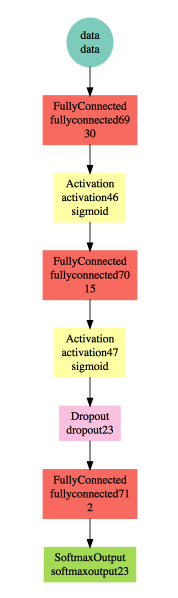
\includegraphics[width=0.2\textwidth]{images/ml/mlp/sigmoid}
	\caption{Architettura dei due modelli addestrati, rispettivamente con 
	funzione di attivazione ReLU e sigmoide.}
	\label{fig:mlp_architecture}
\end{figure}
